% This is "sig-alternate.tex" V2.0 May 2012
% This file should be compiled with V2.5 of "sig-alternate.cls" May 2012
%
% This example file demonstrates the use of the 'sig-alternate.cls'
% V2.5 LaTeX2e document class file. It is for those submitting
% articles to ACM Conference Proceedings WHO DO NOT WISH TO
% STRICTLY ADHERE TO THE SIGS (PUBS-BOARD-ENDORSED) STYLE.
% The 'sig-alternate.cls' file will produce a similar-looking,
% albeit, 'tighter' paper resulting in, invariably, fewer pages.
%
% ----------------------------------------------------------------------------------------------------------------
% This .tex file (and associated .cls V2.5) produces:
%       1) The Permission Statement
%       2) The Conference (location) Info information
%       3) The Copyright Line with ACM data
%       4) NO page numbers
%
% as against the acm_proc_article-sp.cls file which
% DOES NOT produce 1) thru' 3) above.
%
% Using 'sig-alternate.cls' you have control, however, from within
% the source .tex file, over both the CopyrightYear
% (defaulted to 200X) and the ACM Copyright Data
% (defaulted to X-XXXXX-XX-X/XX/XX).
% e.g.
% \CopyrightYear{2007} will cause 2007 to appear in the copyright line.
% \crdata{0-12345-67-8/90/12} will cause 0-12345-67-8/90/12 to appear in the copyright line.
%
% ---------------------------------------------------------------------------------------------------------------
% This .tex source is an example which *does* use
% the .bib file (from which the .bbl file % is produced).
% REMEMBER HOWEVER: After having produced the .bbl file,
% and prior to final submission, you *NEED* to 'insert'
% your .bbl file into your source .tex file so as to provide
% ONE 'self-contained' source file.
%
% ================= IF YOU HAVE QUESTIONS =======================
% Questions regarding the SIGS styles, SIGS policies and
% procedures, Conferences etc. should be sent to
% Adrienne Griscti (griscti@acm.org)
%
% Technical questions _only_ to
% Gerald Murray (murray@hq.acm.org)
% ===============================================================
%
% For tracking purposes - this is V2.0 - May 2012

\documentclass{sig-alternate}

\usepackage{url}
\usepackage[usenames]{xcolor}

\newcommand{\Jose}[1]{{\color{red} [[JOSE:: #1]]}}
\newcommand{\Leo}[1]{{\color{blue} [[LEO:: #1]]}}
\newcommand{\Meng}[1]{{\color{green} [[MENG:: #1]]}}
\newcommand{\Norbert}[1]{{\color{orange} [[NORBERT:: #1]]}}

\begin{document}
%
% --- Author Metadata here ---
\conferenceinfo{SPAA}{'15 Portland, Oregon, USA}
%\CopyrightYear{2007} % Allows default copyright year (20XX) to be over-ridden - IF NEED BE.
%\crdata{0-12345-67-8/90/01}  % Allows default copyright data (0-89791-88-6/97/05) to be over-ridden - IF NEED BE.
% --- End of Author Metadata ---

\title{Succinct Trees Construction on Multicore Architectures}
%\subtitle{[Extended Abstract]
%\titlenote{A full version of this paper is available as
%\textit{Author's Guide to Preparing ACM SIG Proceedings Using
%\LaTeX$2_\epsilon$\ and BibTeX} at
%\texttt{www.acm.org/eaddress.htm}}}
%
% You need the command \numberofauthors to handle the 'placement
% and alignment' of the authors beneath the title.
%
% For aesthetic reasons, we recommend 'three authors at a time'
% i.e. three 'name/affiliation blocks' be placed beneath the title.
%
% NOTE: You are NOT restricted in how many 'rows' of
% "name/affiliations" may appear. We just ask that you restrict
% the number of 'columns' to three.
%
% Because of the available 'opening page real-estate'
% we ask you to refrain from putting more than six authors
% (two rows with three columns) beneath the article title.
% More than six makes the first-page appear very cluttered indeed.
%
% Use the \alignauthor commands to handle the names
% and affiliations for an 'aesthetic maximum' of six authors.
% Add names, affiliations, addresses for
% the seventh etc. author(s) as the argument for the
% \additionalauthors command.
% These 'additional authors' will be output/set for you
% without further effort on your part as the last section in
% the body of your article BEFORE References or any Appendices.

\numberofauthors{4} %  in this sample file, there are a *total*
% of EIGHT authors. SIX appear on the 'first-page' (for formatting
% reasons) and the remaining two appear in the \additionalauthors section.
%
\author{
% You can go ahead and credit any number of authors here,
% e.g. one 'row of three' or two rows (consisting of one row of three
% and a second row of one, two or three).
%
% The command \alignauthor (no curly braces needed) should
% precede each author name, affiliation/snail-mail address and
% e-mail address. Additionally, tag each line of
% affiliation/address with \affaddr, and tag the
% e-mail address with \email.
%
% 1st. author
\alignauthor Jos\'e Fuentes-Sep\'ulveda\\
       \affaddr{Universidad de Concepci\'on}\\
       \affaddr{Edmundo Larenas 219}\\
       \affaddr{Concepci\'on, Chile}\\
       \email{jfuentess@udec.cl}
% 2nd. author
\alignauthor
Leo Ferres\\
       \affaddr{Universidad de Concepci\'on}\\
       \affaddr{Edmundo Larenas 219}\\
       \affaddr{Concepci\'on, Chile}\\
       \email{lferres@udec.cl}
\and  % use '\and' if you need 'another row' of author names
% 3rd. author
\alignauthor Meng He\\
       \affaddr{Dalhousie University}\\
       \affaddr{Mona Campbell 314}\\
       \affaddr{Halifax, Canada}\\
       \email{menghe@dal.ca}
% 4th. author
\alignauthor Norbert Zhe\\
       \affaddr{Dalhousie University}\\
       \affaddr{Mona Campbell 314}\\
       \affaddr{Halifax, Canada}\\
       \email{nzeh@cs.dal.ca}
}

\maketitle
\begin{abstract}

\end{abstract}

% A category with the (minimum) three required fields
\category{}{}{}
%A category including the fourth, optional field follows...
\category{}{}{}[]

\terms{}

\keywords{}

%%%%%%%%%%%%%%%%%%%%%%%%
%%%%% INTRODUCTION %%%%%
%%%%%%%%%%%%%%%%%%%%%%%%

\section{Introduction}
\label{sec:introduction}
Trees are ubiquitous in Computer Science.  They have applications in
every aspect of computing from XML/HTML processing to abstract syntax
trees (AST) in compilers, phylogenetic trees in computational genomics
or shortest path trees in path planning.  The ever increasing amounts
of structured, hierarchical data processed in many applications have
turned the processing of the corresponding large tree structures into
a bottleneck, particularly when they do not fit in memory.  Succinct
tree representations store trees using as few bits as possible and
thereby significantly increase the size of trees that fit in memory
while still supporting important primitive operations in constant
time.  There exist such representations that use only $2n - \Theta(\lg
n)$ bits\footnote{We use $\lg x$ to mean $\log_{2}x$ throughout this
paper.} to store the topology of a tree with $n$ nodes, which is close
to the information-theoretic lower bound and much less than the space
used by traditional pointer-based representations.

Alas, the construction of succinct trees is quite slow compared to the
construction of pointer-based representations.  Multicore parallelism
offers one possible tool to speed up the construction of succinct
trees, but little work has been done in this direction so far.  The
only results we are aware of focus on the construction of Wavelet
trees, which are used in representations of text indexes.  In
\cite{Fuentes2014}, two practical multicore algorithms for Wavelet
tree construction were introduced.  Both algorithms perform $O(n\lg
\sigma)$ work and have span $O(n)$, where $n$ is the input size and
$\sigma$ is the alphabet size.  In \cite{DBLP:journals/corr/Shun14},
Shun introduced three new algorithms to construct Wavelet trees in
parallel.  The in practice best algorithm performs $O(n\lg \sigma)$
work and has span $O(\lg n\lg \sigma)$.  Shun also explained how to
parallelize the construction of rank/select structures so it requires
$O(n)$ work and $O(1)$ span for rank structures, and $O(n)$ work and
$O(\lg n)$ span for select structures.

In this paper, we provide a parallel algorithm that constructs the
{\tt RMMT} tree representation of
\cite{Navarro:2014:FFS:2620785.2601073} in $O(n/p + \lg p)$ time
using $p$ cores.  This structure uses $2n + o(n)$ bits to store an
ordinal tree with $n$ nodes and supports a rich set of basic
operations on these trees in $O(\lg n)$ time.  While this query time
is theoretically suboptimal, the {\tt RMMT} structure is simple enough
to be practical and has been verified experimentally to be very small
and support fast queries in practice~\cite{ACNSalenex10}.  Combined
with the fast parallel construction algorithm presented in this paper,
it provides an excellent tool for manipulating very large trees in
many applications.

We implemented and tested our algorithm on a number of real-world input trees
having billions of nodes.
Our experiments show that our algorithm run on a single core is competitive with
state-of-the-art sequential constructions of the {\tt RMMT} structure and
achieves good speed-up on up to 64 cores and likely beyond.

\ignore{The remainder of this paper is organized as follows:
Section~\ref{sec:relwork} gives a brief overview of the {\tt RMMT}
structure, to clearly define its structure and illustrate how it can
be used to support basic operations on trees efficiently.  It also
briefly discusses other previous work on succinct tree representations
and reviews the dynamic multithreading model, which we use to analyze
the theoretical running time of our algorithm.
Section~\ref{sec:multicoreST} describes our parallel algorithm for
constructing the {\tt RMMT} structure.  Section~\ref{sec:exps}
discusses our experimental setup and results.
Section~\ref{sec:conclusion} offers concluding remarks and discusses
future work.}

%%% Local Variables:
%%% mode: plain-tex
%%% TeX-master: t
%%% End:



%%%%%%%%%%%%%%%%%%%%%%%%
%%%%% RELATED WORK %%%%%
%%%%%%%%%%%%%%%%%%%%%%%%

\section{Related Work}
\label{sec:relwork}
\Jose{Here we should introduce the Range Min-Max Tree}

\subsection{Succinct Trees}
\label{subsec:suctrees}
Jacobson~\cite{j1989} first proposed to design succinct data structures.
He showed how to represent an ordinal trees on $n$ nodes using $2n+o(n)$ bits so
that computing the first child, the next sibling or the parent of any given node
takes $O(\lg n)$ time in the bit probe model.
Clark and Munro~\cite{cm1996} showed how to support the same operations in
constant time in the word RAM model with word size $\Theta(\lg n)$.
Since then, a lot of work has been done on succinct tree representations, to
support more navigational operations, to achieve compression, to provide support
for update operations, and so
on~\cite{mr1997,bdmr1999,grr2004,jss2007,ly2008,hms2012,fm2014,Navarro:2014:FFS:2620785.2601073}. 
Raman and Rao~\cite{rr2013} give a thorough survey of the state of the art.

In this paper, we present a parallel algorithm to construct the succinct tree
representation proposed recently by Navarro and
Sadakane~\cite{Navarro:2014:FFS:2620785.2601073}, referred to as
NS-representation throughout this paper.
This representation is the first to achieve a {\em redundancy}
of $O(n/\lg^c n)$ bits for any positive constant $c$.
The redundancy is the additional space used by the data structure above the
information-theoretic lower bound.
While all previous tree representations achieved a redundancy of $o(n)$ bits,
their redundancy was $\Omega(n \lg\lg n / \lg n)$ bits, that is, just slightly
sub-linear.
The NS-representation also supports a large number of
navigational operations in constant time (see Table~\ref{tbl:operations}); only
the work in \cite{hms2012,fm2014} supports two more operations.
The main reason we focus on this representation in this paper is an experimental
study on succinct trees~\cite{ACNSalenex10}, which showed that an implementation
of a simplified version ofthe NS-representation uses less space than other
existing representations in most cases and performs most operations faster.
Our goal in this paper is to alleviate the construction bottleneck of this
representation by exploiting multicore parallelism.

\begin{table}[t]
\begin{center}
\begin{tabular}{|>{\raggedright}p{2.4cm}|>{\raggedright\arraybackslash}p{5.2cm}|} \hline
\bf Operation                         & \bf Description        \\ \hline
$\child(x,i)$                         & Report $i$th child of node $x$\\
$\childrank(x)$                       & Report number of left siblings of node $x$\\
$\degree(x)$                          & Report degree of node $x$\\
$\depth(x)$                           & Report depth of node $x$\\
$\levelanc(x,i)$                      & Find ancestor of node $x$ that is $i $levels above node $x$ \\
$\subtreesize(x)$                     & Report number of nodes in the subtree rooted at node $x$ \\
$\height(x)$                          & Report height of the subtree rooted at $x$ \\
$\deepestnode(x)$                     & Find deepest node in the subtree rooted at node $x$\\
$\lca(x,y)$                           & Find lowest common ancestor of nodes $x$ and $y$ \\
$\lmostleaf(x)$ /$\rmostleaf(x)$      & Find leftmost/rightmost leaf of the subtree rooted at node $x$\\
$\leafrank(x)$                        & Report Number of leaves before node $x$ in preorder\\
$\leafselect(i)$                      & Find $i$th leaf from left to right\\
$\prerank(x)$ /$\postrank(x)$         & Report number of nodes preceding node $x$ in preorder/postorder\\
$\preselect$ /$\postselect(i)$        & Find $i$th node in preorder/postorder\\       
$\levellmost(i)$ /$\levelrmost(i)$    & Find leftmost/rightmost node among all the nodes at depth $i$ \\
$\levelsucc(x)$ /$\levelpred(x)$      & Find node immediately to the left/right of node $x$ among nodes at the same depth\\ \hline
$\access(i)$                          & Report the $i$th parenthesis $P[i]$        \\ 
$\findopen(i)$ /$\findclose(i)$       & Find the matching parenthesis of $P[i]$ \\
$\enclose(i)$                         & Find the closest enclosing matching parenthesis pair for $P[i]$ \\
$\rankopen(i)$ /$\rankclose(i)$       & Report the number of opening/closing parentheses in $P[1..i]$\\
$\selectopen(i)$ /$\selectclose(i)$   & Find the $i$th opening/closing parenthesis\\ \hline
\end{tabular}
\caption{Operations supported by the NS-representation, including operations
  on the corresponding balanced parenthesis sequence.}
\label{tbl:operations}
\end{center}
\end{table}

The NS-representation is based on the balanced parenthesis sequence $P$ of
the input tree, which is obtained by performing a preorder traversal
of the given tree and writing down an opening parenthesis when visiting
a node for the first time and a closing parenthesis after visiting
all its descendants.
Thus, the length of $P$ is $2n$.
The parenthesis sequence of the ordinal tree in Figure~\ref{figure:bp}, for
example, is $P = ((())((()())(()(())))()())$.

\begin{figure}
  \centering
  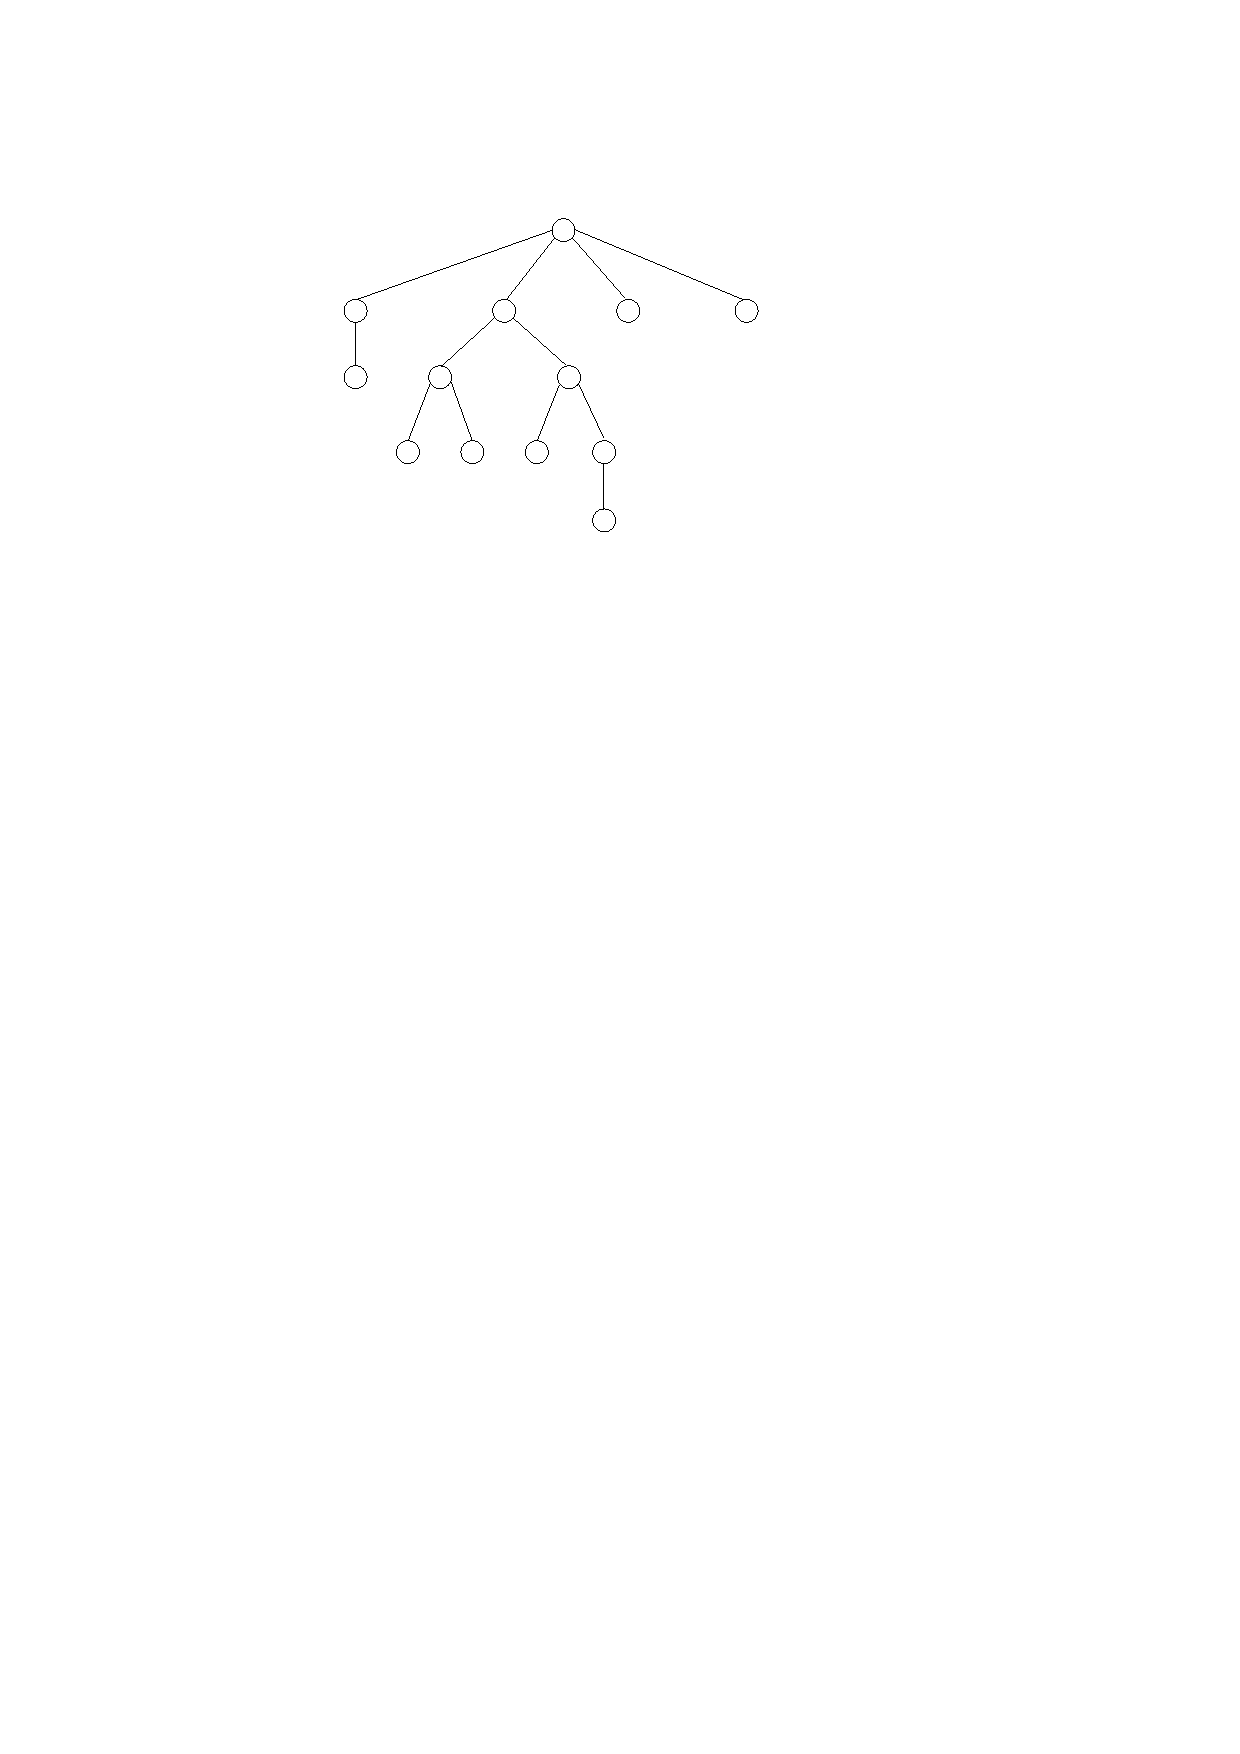
\includegraphics[scale=0.5]{images/bp.pdf}
  \caption{An ordinal tree used as an example.}
  \label{figure:bp}
\end{figure}

The NS-representation is not the first structure to use balanced parentheses to
represent trees.
Munro and Raman~\cite{mr1997} were the first to design succinct representations
of balanced parentheses and used them to represent ordinal trees succinctly by
reducing a set of navigational operations on trees to operations on their
balanced parenthesis sequences.
Their solution supports only a subset of the operations listed in
Table~\ref{tbl:operations}.
Additional operations can be supported using  auxiliary data
structures~\cite{ly2008}.
To support all operations in Table~\ref{tbl:operations}, many auxiliary data
structures are required, which add to the size of the final data structure
and make it complex in both theory and practice.
The main novelty of Navarro and Sadakane's
work~\cite{Navarro:2014:FFS:2620785.2601073} lies in the strategy they used to
reduce a large set of operations on trees and balanced parenthesis sequences to
a small set of \emph{primitive operations}.
Representing $P$ as a bit vector storing a $1$ for each opening parenthesis
and a $0$ for each closing parenthesis, these primitive operations are the
following.
Here, $g$ is an arbitrary function on $\{0,1\}$.
\begin{align*}
\sumop(P,g,i,j) &= \textstyle\sum_{k=i}^jg(P[k])\\
\fwdsearch(P,g,i,d) &= \min\{j \mid j \ge i, \sumop(P,g,i,j) = d\}\\
\bwdsearch(P,g,i,d) &= \max\{j \mid j \le i, \sumop(P,g,j,i) = d\}\\
\rmq(P,g,i,j) &= \min\{\sumop(P,g,i,k) \mid i\le k\le j\}\\
\RMQ(P,g,i,j) &= \max\{\sumop(P,g,i,k) \mid i\le k\le j\}\\
\rmqi(P,g,i,j) &= \argmin_{k\in[i,j]}\{\sumop(P,g,i,k)\}\\
\RMQi(P,g,i,j) &= \argmax_{k\in[i,j]}\{\sumop(P,g,i,k)\}
\end{align*}
Navarro and Sadakane defined three functions on $[0,1]$:
\begin{align*}
  \pi  &: 1 \mapsto 1\quad 0 \mapsto -1\\
  \phi &: 1 \mapsto 1\quad 0 \mapsto 0\\
  \psi &: 1 \mapsto 0\quad 0 \mapsto 1
\end{align*}
Most of the operations in Table~\ref{tbl:operations} can then be supported using
the primitive operations by setting $g$ to be $\pi$, $\phi$ or~$\psi$.
For example, $\findclose(i) = \fwdsearch(P,\pi,i,0)$.
Thus, it suffices to support the operations in Table~\ref{tbl:operations} for
$g = \pi$, $g = \phi$ or $g = \psi$, as well as a few navigational operations
that cannot expressed using these primitive operations, which are $\degree$,
$\child$, $\childrank$ and the four operations in Table~\ref{tbl:operations}
related to leaf nodes.
To support the primitive operations, Navarro and Sadakane designed a simple data
structure called \emph{Range Min-Max Tree} ({\tt RMMT}) (see next subsection).
It supports the primitive operations in logarithmic time when used to represent
the entire sequence~$P$.
To achieve constant-time operations, $P$ is further partitioned into chunks.
Each chunk is represented using a {\tt RMMT}, which can support primitive
operations inside the chunk in constant time if the chunk is small enough.
Additional data structures are used to support operations on the entire sequence
$P$ in constant time.

\subsubsection{The Range Min-Max Tree}

Let $w$ denote the number of bits in a word.
The range min-max tree ({\tt RMMT}) is designed to support the primitive
operations for functions $\pi$, $\phi$, and $\psi$.
We first describe how to construct a {\tt RMMT} for the function $\pi$ and
later show how it can be easily augmented to support the primitive operations
for the other two functions.
Recall that $T$ denotes the input tree on $n$ nodes, and $P$ represents its
balanced parenthesis sequence, where $P[i] = 1$ iff the $i$th
parenthesis is an opening parenthesis.
To define the {\tt RMMT}, we partition $P[1..2n]$ into disjoint chunks of
a size $s \le w/2$ to be chosen later.
For simplicity, we assume that the length of $P$ is a multiple of~$s$.
The {\tt RMMT} is a complete $k$-ary tree over the sequence of these chunks,
for some \emph{arity} $k \ge 2$ to be chosen later (see
Figure~\ref{fig:RangeMinMaxTree}).

Next define the following five arrays $E$, $e$, $m$, $M$, and $n^*$.
These arrays are only used in the description and are not stored explicitly
in the data structure.
The {\em excess} at position $i$ of $P$ is defined as $\sumop(P,\pi,0,i) =
\sum_{k=0}^{i} \pi(P[k])$.
$E$ has length $2n$ and $E[i]$ is the excess at position $i$.
The other four arrays are of length $2n/s$ each.
$e[i]$ stores the excess at position $is$, that is, at the end of the $i$th
chunk.
$m[i]$ and $M[i]$ store the minimum and maximum excess at any position in the
$i$th chunk, respectively.
$n^*[i]$ stores the number of positions in the $i$th chunk that have the
minimum excess value $m[i]$.
Each internal node, $u$, of the {\tt RMMT} also stores four similar values
$e[u]$, $m[u]$, $M[u]$, and $n^*[u]$, which have the same meaning as defined
above with respect to the subsequence of $P$ that is the concatenation of the
chunks corresponding to descendant leaves of $u$.
These values are illustrated in Figure~\ref{fig:RangeMinMaxTree}.
As the {\tt RMMT} is a complete tree, we do not store its structure explicitly.
Instead, we can simply store the values associated with its nodes in four arrays
$e'$, $m'$, $M'$, and $n'$ indexed like a $k$-ary heap.

\begin{figure}[t]
  \centering
  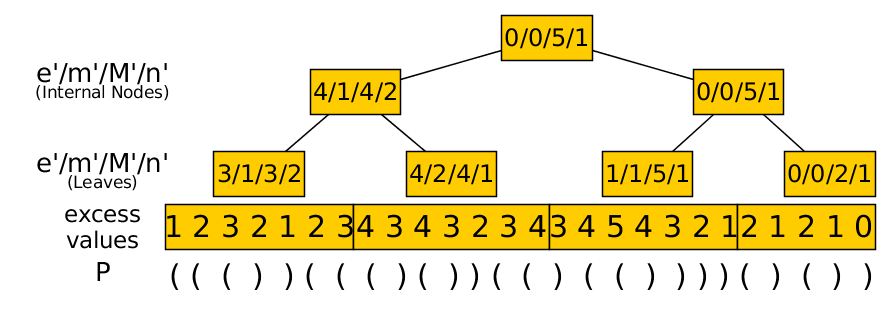
\includegraphics[scale=0.18]{./images/Range-min-max-tree.png}
  \caption{Range min-max tree}
  \label{fig:RangeMinMaxTree}
\end{figure}

Combined with a standard succinct data structure technique called {\em table
  lookup}, a {\tt RMMT} can support the primitive operations for $\pi$, as well
as $\degree$, $\child$ and $\childrank$ queries.
For example, consider $\fwdsearch(P,\pi,i,d)$.
We first check the chunk containing $P[i]$ to see if the answer is inside the
same chunk.
This can be done in constant time by constructing a universal lookup table whose
content does not depend on $P$: For each possible bit vector of length $s$,
and each of the $s$ position in the bit vector, we store the answer of
$\fwdsearch(P,\pi,i,d)$ if it can be found inside this bit vector, or $-1$
otherwise.
As there are $2^s$ bit vectors of length $s$, this table uses
$2^s\poly(s)$ bits.
If we find the  answer by performing a table lookup for the chunk containing
$P[i]$, then we return.
Otherwise, we search among the $m$ and $M$ values of the right siblings of the
leaf node $u$ corresponding to this chunk, to find the closest right sibling
that contains the answer if the answer is within chunks represented by these
siblings.
If the $m$ and $M$ values of the $k$ children of each internal node can be
packed into $O(w)$ bits, i.e., $k \lg n = O(w)$, then we can again construct
universal lookup tables for internal nodes to perform this step in constant
time.
We repeat this process until we find a right sibling, $v$, of an ancestor of $u$
whose corresponding substring of $P$ contains the answer.
We then use a similar idea to descend down the tree starting from $v$ to look
for the leaf descendant of $v$ containing the result.
Thus, we can support $\fwdsearch$ in $O(h)$ time, where $h$ is the height of the
{\tt RMMT}, provided that $k \lg n = O(w)$.

To support the primitive operations for functions $\phi$ and~$\psi$, we can
define six arrays $e'_{\phi}$, $m'_{\phi}$, $M'_{\phi}$, $e'_{\psi}$,
$m'_{\psi}$ and $M'_{\psi}$ which are similar to $e'$, $m'$ and $M'$ defined for
$\pi$ ($n'$ is defined to support $\degree$, $\child$ and $\childrank$ only, so
we need not define similar arrays for $\phi$ and $\psi$).
We make use of the following three observations to avoid storing these six
arrays explicitly: $\sumop(P, \phi, 0, i)$ and $\sumop(P, \psi, 0, i)$ are
nondecreasing, $\sumop(P, \phi, 0, i) + \sumop(P, \psi, 0, i) = i$ and
$\sumop(P, \phi, 0, i) - \sumop(P, \psi, 0, i) = \sumop(P, \pi, 0, i)$.
Thus, the each value in these six arrays can be computed in constant time
without storing them explicitly.
We only need to store the universal tables needed to support primitive
operations for $\phi$ and $\psi$.

To support $\leafrank$, $\leafselect$, $\lmostleaf$ and\break $\rmostleaf$, we
define a conceptual bit vector $P_1[1..2n]$ in which $P_1[i] = 1$ iff $P[i] = 1$
and $P[i+1] = 0$.
Hence each $1$-bit in $P_1$ corresponds to a leaf node.
The above operations then reduce to $\rankop$ and $\selop$ operations on
$P_1$, where $\rankop(P_1, i)$ returns the number of $1$s in $P_1[1..i]$ and
$\selop(P_1, i)$ returns the position of the $i$th $1$-bit in $P_1$.
For example, we have $\leafrank = \rankop(P_1, i)$.
$\rankop$ and $\selop$ operations can be further reduced to $\sumop$ and
$\fwdsearch$ for the function $\phi$ on $P_1$, which can be supported using
another range min-max tree.
Since any $O(w)$ bits in the sequence $P_1$ can be computed from $P$ in constant
time using table lookup, $P_1$ itself need not be stored explicitly, while the
cost of storing the information for the internal nodes of this range min-max
tree is dominated by the space usage of the range min-max tree for $P$.

To analyze the space usage of the entire data structure, we observe that if we
store $P$, $e'$, $m'$, $M'$ and $n'$ explicitly in a straightforward manner, the
space usage  would be $2n + \frac{k}{k-1} \cdot \frac{n}{s} \cdot \lg n$.
Navarro and Sadakane commented that choosing $s = w/2$ and $k = w / \lg n$ gives
a simple structure supporting all the operations in Table~\ref{tbl:operations}
in $O(\lg n)$ time.
However, if the trees are large enough that $w = \Theta(\lg n)$, then $e'$,
$m'$, $M'$ and $n'$ would occupy $O(n)$ bits, and the size of the representation
would be greater than is typical for a succinct tree representation,
which would use $2n+o(n)$ bits.
To reduce the overall space cost to $2n+o(n)$ bits, we can set
$s = \lceil w\lg n\rceil$ and $k = 2$.
With these parameters, looking for a potential answer to a query within a chunk
requires $O(\lg n)$ table lookups, which is dominated by the $O(\lg n)$ cost of
traversing the tree to answer queries.
Thus, the overall query cost remains $O(\lg n)$.
Moreover, for $k = 2$, universal tables are not needed for internal nodes.
Thus, we have the following lemma:

\begin{lemma}\label{lem:lg}
  An ordinal tree and its balanced parentheses sequence can be represented using
  range min-max trees in $2n + o(n)$ bits, where $n$ is the number of nodes in
  the tree.
  This structure supports all operations in Table~\ref{tbl:operations} in
  $O(\lg n)$ time.
\end{lemma}

Navarro and Sadakane showed how to use the structure described so far as a
building block for a more complicated structure that supports all operations in
Table~\ref{tbl:operations} in constant time.
Due to its complexity, however, this structure is much more difficult to
implement and may not be efficient in practice.
On the other hand, the structure described here has been experimentally verified
to be very small and achieve very good query performance in
practice~\cite{ACNSalenex10}.
This is the reason we chose this structure as the basis for our work presented
in this paper.

\subsection{Dynamic Multithreading Model}
\label{subsec:dym}
{\em Dynamic multithreading} (DYM) \cite[Chapter~27]{Cormen2009} is a
model of parallel computation that is faithful to several industry standards
such as Intel's CilkPlus (\url{cilkplus.org}), OpenMP Tasks
(\url{openmp.org/wp}), and Threading Building
Blocks (\url{threadingbuildingblocks.org}).

In this model, a {\em multithreaded computation} is modelled as a directed
acyclic graph (DAG) $G=(V,E)$ where the set of vertices $V$ are instructions
and $(u,v) \in E$ if $u$ must be executed before $v$.\footnote{Notice that the
  RAM model is a subset of the DYM model where the outdegree of every
  vertex $v \in V$ is $\leq 1$.\Norbert{Why ``$\le$''?  Doesn't the strictly
    sequential nature of the RAM model mean that everybody except the first and
    last vertices has exactly one in-neighbour and one out-neighbour?}}
The time $T_p$ needed to execute the computation on $p$ processors depends on
two parameters of the computation: its {\em work} $T_1$ and its {\em span}
$T_\infty$.
Assuming each instruction takes constant time, the work is simpy the number of
nodes (i.e., instructions) in $G$.
Since each instruction takes constant time, it clearly takes $\Theta(T_1)$ time
to execute $G$ on a single processor.
More generally, $p$ processors can execute only $p$ instructions at a time, so
$T_p = \Omega(T_1/p)$.
The span is the length of the longest path in $G$.
Since the instructions on this path need to be executed one after another, no
matter how many processors we have at our disposal, we also have
$T_p = \Omega(T_\infty)$.
Together, these two lower bounds give $T_p = \Omega(T_\infty + T_1/p)$ and
work-stealing schedulers match this lower bound to within a constant factor
(to within a factor 2 from the optimal
performance)~\cite{Blumofe:1999:SMC:324133.324234}.
The degree to which an algorithm can take advantage of the presence of $p > 1$
processors is captured by its {\em speed-up} $T_1 / T_p$ and its
{\em parallelism} $T_1 / T_\infty$.
In the absence of cache effects, the best speed-up one can hope for is $p$,
also known as {\em linear speed-up}.
The parallelism provides an upper bound on the achievable speed-up independent
of the number of available processors.

In order to describe parallel algorithms in the DYM model, we augment sequential
pseudocode with three special keywords.
The {\bf spawn} keyword, followed by a procedure call, indicates that the
procedure should run in its own thread and {\em may} thus be executed in
parallel to the thread that spawned the procedure call.
The {\bf sync} keyword indicates that the current thread must wait for the
termination of all the threads it has spawned before proceeding.
It thus provides a simple barrier-style synchronization mechanism.
Finally, {\bf parfor} is ``syntactic sugar'' for {\bf spawn}ing one thread per
iteration in a for loop, thereby allowing these iterations to run in parallel,
followed by a {\bf sync} operation that waits for all iterations to complete.
In practice, the overhead is logarithmic in the number of iterations.
If a procedure exits, either implicitly or explicitly using a {\bf return}
statement, it implicitly performs a {\bf sync} to ensure all threads it spawned
finish first.
\Norbert{Got rid of the ``strand'' stuff.
  It seems a technicality relevant only to the operation of work-stealing
  schedulers.
  If we actually use it in the analysis of the algorithm in Section 3, we
  may have to bring it back.}

\subsection{Multicore succinct data structures}
\label{subsec:multicoreSDS}
A weak point of succinct data structures is their construction time,
which is generally quite slow compared to the construction time of
traditional ``pointer-linked'' data structures. We have been working
on improving construction time for succinct data structures
\cite{Fuentes2014}. In that paper, two practical multicore algorithms
for wavelet tree construction were introduced. Both algorithms run
have $O(n\lg \sigma)$ {\em work} time and $O(n)$ {\em span}, where $n$
is the input size and $\sigma$ is the alphabet size. In
\cite{DBLP:journals/corr/Shun14}, Shun introduced 3 new algorithms to
construct wavelet trees in parallel. The best algorithm, in practice,
has $O(n\lg \sigma)$ {\em work} time and $O(\lg n\lg \sigma)$ {\em
span}. Shun also explain how to parallelize the construction of
rank/select structures, taking $O(n)$ {\em work} time and $O(1)$ {\em
span} for rank structures and $O(n)$ {\em work} time and $O(\lg n)$
{\em span} for select structures. The author does not provide an
implementation of its proposal.

%%%%%%%%%%%%%%%%%%%%%%%%%%%%%%%%%%%
%%%%% MULTICORE SUCCINCT TREE %%%%%
%%%%%%%%%%%%%%%%%%%%%%%%%%%%%%%%%%%

\section{Multicore Succinct Tree}
\label{sec:multicoreST}
% We will focus on polylogarithmic-size trees because they are the
% only ones that have an implementation we can compare ourselves to;
% in particular, we take the {\tt
% libcds}\footnote{\url{http://libcds.recoded.cl}. We thank Diego
% Arroyuelo for the conversations about the implementation of succinct
% trees.}\cite{ACNSalenex10} and {\tt
% sdsl}\footnote{\url{https://github.com/simongog/sdsl-lite}}
% libraries as state-of-the-art and our sequential baseline.
%
% \Jose{In this section I'll use the same notation used in
% \cite{Navarro:2014:FFS:2620785.2601073}. This notation should be
% introduced in the Related Work section}\\



%%%%%%%%%%%%%%%%%%%%%%%
%%%%% EXPERIMENTS %%%%%
%%%%%%%%%%%%%%%%%%%%%%%

\section{Experimental Results}
\label{sec:exps}
To evaluate the performance of our {\tt PSTA} algorithm, we compare it against
{\tt libcds}~\cite{libcds} and {\tt sdsl}~\cite{sdsl}, which are
state-of-the-art implementations of the {\tt RMMT}.
Both assume that the input tree is given as a parenthesis sequence, as we do
here.
Our implementation of the {\tt PSTA} algorithm deviates from the description in
Section~\ref{sec:multicoreST} in that the prefix sum computation in
line~22 of the algorithm is done sequentially in our implementation.
This changes the running time to $O(n/p + p)$ but simplifies the implementation.
Since $p \ll n/p$ for the input sizes we are interested in and the numbers of
cores available on current multicore systems, the impact on the running
time is insignificant.


%%%%%%%%%%%%%%%%%%%%%%
%%%%% CONCLUSION %%%%%
%%%%%%%%%%%%%%%%%%%%%%

\section{Conclusion}
\label{sec:conclusion}
In this work we shown that it is possible to improve the construction time of succinct
trees, exploiting current multicore architectures. We introduce a practical algorithm that
achieves $O(\frac{n}{p}+\lg p)$ construction time, to a tree with $n$ nodes and $p$
threads, while supports a rich set of navigational operations in $O(\lg n)$ time. This
practical algorithm was tested against state-of-the-art libraries, reaching good speedup.
We also proposed other algorithm to a more complex succinct tree representation, with
$O(\frac{n\lg p}{p})$ construction time, which supports navegational operations in
constant time. Since our algorithms need, as input, a tree stored as a parentheses
sequence, we presented an algorithm to compute such parentheses sequence in parallel in
$O(\frac{n}{p}+\lg p)$ time.

In this paper we focused on static representation of succinct trees. However, our results
may be the base to the parallel construction of dynamic succinct trees, as the dynamic
succinct trees of \cite{Navarro:2014:FFS:2620785.2601073}. Also, it would be interesting
to study how to extend our results to succinct representation of \emph{labeled} trees. We
shall explore the extension of our results to the parallel construction other succinct
data structures that use succinct trees representations as part of their representations.
Such is the case of succinct planar graphs. Note that we can use the results of
\cite{Fuentes2014} to parallelize batches of navigational operations, reaching a good
pratical speedup. Since that the \emph{range min-max tree}, that our algorithms construct,
is a complete tree, the strategy underlying our algorithms can be applied to construct
general complete trees in parallel.

We believe that exploit current multicore architectures to improve the overall performance
of succinct data structures is a interesting research line. Taking the features of
succinct data structures and the processing power of multicore architectures allows to
design practical data structures with competitive querying time, efficient space usage and
fast/scalable construction time.

%ACKNOWLEDGMENTS are optional
\section{Acknowledgments}
This section is optional; it is a location for you
to acknowledge grants, funding, editing assistance and
what have you.  In the present case, for example, the
authors would like to thank Gerald Murray of ACM for
his help in codifying this \textit{Author's Guide}
and the \textbf{.cls} and \textbf{.tex} files that it describes.

%
% The following two commands are all you need in the
% initial runs of your .tex file to
% produce the bibliography for the citations in your paper.
\bibliographystyle{abbrv}
\bibliography{sigproc}  % sigproc.bib is the name of the Bibliography in this case
% You must have a proper ".bib" file
%  and remember to run:
% latex bibtex latex latex
% to resolve all references
%
% ACM needs 'a single self-contained file'!
%
\end{document}
